\documentclass[11pt]{article}

\usepackage{amsmath}
\usepackage{amsfonts}
\usepackage{amssymb}

% Give ourself extra space for text
\usepackage[left = 2.2cm, right = 2.2cm, top = 1.8cm, bottom = 2.8cm]{geometry}

% Allows us to easily change the numbering system used in things like \begin{enumerate}. https://ctan.org/tex-archive/macros/latex/contrib/enumitem/
\usepackage[shortlabels]{enumitem}

% Turns table of contents, \refs, etc. into hyperlinks
\usepackage{hyperref}

% To include image, just use \includegraphics[scale=•]{relative path to image}
\usepackage{graphicx}
\graphicspath{ {./images/} }

% Common sets
\newcommand{\integers}{\mathbb{Z}}
\newcommand{\naturals}{\mathbb{N}}
\newcommand{\reals}{\mathbb{R}}

% Power set
\newcommand{\powerset}{\mathcal{P}}

% Identity matrix
\newcommand{\ident}{\mathbb{I}}

% Inverse hyperbolic functions
\DeclareMathOperator{\arcosh}{arcosh}
\DeclareMathOperator{\arsinh}{arsinh}
\DeclareMathOperator{\artanh}{artanh}

% I hat, J hat, K hat
\newcommand{\ihat}{\boldsymbol{\hat{\textbf{\i}}}}
\newcommand{\jhat}{\boldsymbol{\hat{\textbf{\j}}}}
\newcommand{\khat}{\boldsymbol{\hat{\textbf{k}}}}

% Better vectors (for single characters)
\renewcommand{\vec}[1]{\mathbf{#1}}

% Allows us to number equations in \begin{align} statements, etc.
\newcommand\numberthis{\addtocounter{equation}{1}\tag{\theequation}}

% Augmented matrices: this allows us to make augmented matrics using something like \begin{bmatrix}[cc|c]. Taken from Stefan Kottwitz at https://tex.stackexchange.com/questions/2233/whats-the-best-way-make-an-augmented-coefficient-matrix.
\makeatletter
\renewcommand*\env@matrix[1][*\c@MaxMatrixCols c]{%
  \hskip -\arraycolsep
  \let\@ifnextchar\new@ifnextchar
  \array{#1}}
\makeatother

% NOTE: This means \section does NOT number sections, but ensures that they appear in the table of contents, which does not occur if simply \section* is used. From egreg @ https://tex.stackexchange.com/a/30225.
\setcounter{secnumdepth}{0} % sections are level 1

\begin{document}
\title{ENG1005: Lecture 23}
\author{Lex Gallon}
\maketitle

\tableofcontents

\section*{Video link}
Click \href{https://echo360.org.au/lesson/G_32340f5d-ff38-43d2-be9d-d88ddb1b3611_b944cecf-8ba5-40d3-a870-0243a0a9e78c_2020-05-13T14:58:00.000_2020-05-13T15:53:00.000/classroom#sortDirection=desc}{here} for a recording of the lecture.

\section{Chain rule - continued}

\subsection{Example}
Show that
\[ \frac{d}{dt} \int_{a(t)}^{b(t)} F(s, t)\, ds = b'(t) F(b(t), t) - a'(F(a(t), t) + \int_{a(t)}^{b(t)} \frac{\partial F}{\partial t} (s, t)\, ds \]

\subsection{Solution}
Define
\[ G(x, y, t) = \int_x^y F(s, t) \, ds \]

\begin{align*}
\frac{\partial G}{\partial x} (x, y, t) &= \frac{\partial}{\partial x} \left( -\int_y^x F(s, t)\, ds \right) \\
&= -F(x, t)
\end{align*}
This comes from the fact that
\[ \frac{d}{dx} \int_c^x f(s)\, ds = f(x) \]
Similarly,
\[ \frac{\partial G}{\partial y}(x, y, t) = \frac{\partial}{\partial y} \left( \int_x^y F(s, t)\, ds \right) = F(y, t) \]
and
\[ \frac{\partial G}{\partial t}(x, y, t) = \frac{\partial}{\partial t} \left( \int_x^y F(s, t)\, ds \right) = \int_x^y \frac{\partial F}{\partial t}(s, t)\,  ds \]
Note that last movement of the derivative inside the integral does not always work, but does in this case so don't worry about it.

So by the chain rule, we have 
\begin{align*}
\frac{d}{dt} \int_{a(t)}^{b(t)} F(s, t)\, dt &= \frac{d}{dt} \left(G(a(t), b(t), t) \right) \\
&= \frac{\partial G}{\partial x}(a(t), b(t), t) a'(t) + \frac{\partial G}{\partial y}(a(t), b(t), t) b'(t) + \frac{\partial G}{\partial x}(a(t), b(t), t) \\
&= -F(a(t), t) a'(t) + F(b(t), t) b'(t) + \int_{a(t)}^{b(t)} \frac{\partial F}{\partial t}(s, t)\, ds
\end{align*}

\section{Directional derivatives and gradients}
\subsection{Definition}
The directional derivative of a function $f(x, y)$ of two variables at a point $(x_0, y_0) \in \reals^2$ in the direction of $\vec{u} = (u_1, u_2) \in \reals^2$ is defined by
\[ D_\vec{u} f(x_0, y_0) = \frac{d}{ds} f(\gamma (s))|_{s=0} \]
where
\[ \gamma(s) = (x_0, y_0) + s \vec{\hat{u}} \quad \left( \vec{\hat{u}} = \frac{\vec{u}}{|\vec{u}|} \right) \]
I.e, $\gamma(s)$ is a line that goes in the direction of $\vec{u}$.

\begin{center} 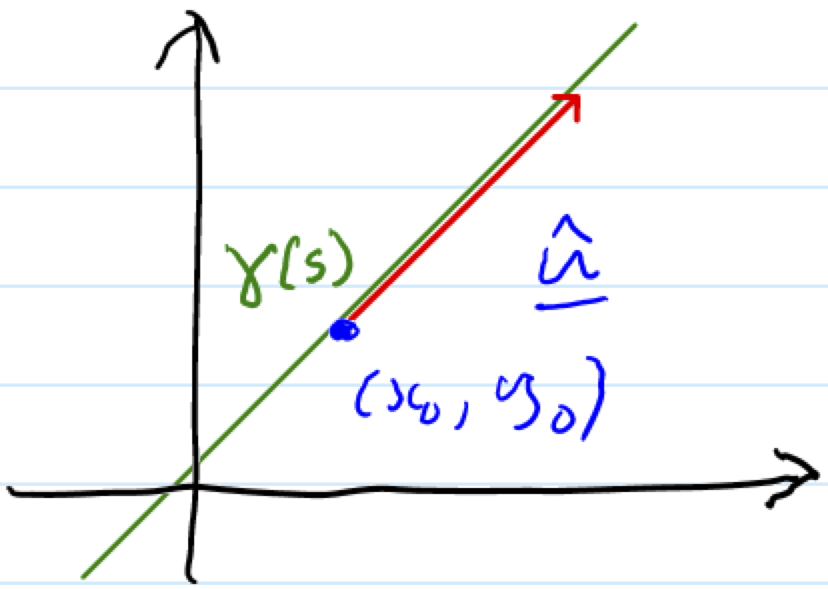
\includegraphics[scale=1]{gamma_line} \end{center}

So,\\
if 
\[ \vec{\hat{u}} = (\hat{u}_1, \hat{u}_2) \]
then 
\[ \gamma(s) = (x(s), y(s)) \]
where 
\[ x(s) = x_0 + \hat{u}_1 s, \quad y(s) = y_0 + \hat{u}_2 s \]
Then
\[ D_\vec{u}f(x_0, y_0) = \frac{d}{ds} f(x(s), y(s)) |_{s=0} \]

\subsection{Definition}
The gradient of a differentiable function $f(x, y)$ of two variables at the point $(x_0, y_0) \in \reals^2$ is defined as
\[ \nabla f(x_0, y_0) = \left( \frac{\partial f}{\partial x}(x_0, y_0), \frac{\partial f}{\partial y}(x_0, y_0) \right) \]

\subsection{Meaning of the directional derivative}
The directional derivative $D_\vec{u}f(x_0, y_0)$ measures the rate of change of the function $f(x, y)$ at the point $(x_0, y_0)$ in the direction of the vector $\vec{u} = (u_1, u_2)$.
\[ |D_\vec{u}f(x_0, y_0)| \equiv \text{ rate of change  of } f(x, y) \text{ at } (x_0, y_0) \text{ in the direction of } \vec{u} = (u_1, u_2). \]
\[ D_\vec{u}f(x_0, y_0) > 0 \Rightarrow f \text{ is } \textbf{increasing} \text{ at } (x_0, y_0) \text{ in the direction of } \vec{u}. \]
\[ D_\vec{u}f(x_0, y_0) < 0 \Rightarrow f \text{ is } \textbf{decreasing} \text{ at } (x_0, y_0) \text{ in the direction of } \vec{u}. \]

\subsection{Relationship between the gradient and the directional derivative}
\subsubsection{Theorem}
If $f(x, y)$ is differentiable at $(x_0, y_0)$ and $\vec{u} = (u_1, u_2)$ is a vector in $\reals^2$, then
\[ D_\vec{u}f(x_0, y_0) = \vec{\hat{u}} \cdot \nabla f(x_0, y_0) \]

\subsubsection{Proof}
Let 
\[ \vec{\hat{u}} = (\hat{u}_1, \hat{u}_2) \]
and
\[ x(s) = x_0 + \hat{u}_1 s \text{ and } y(s) = y_0 + \hat{u}_2  \]
Then
\begin{align*}
D_\vec{u} f(x_0, y_0) &= \frac{d}{ds} f(x(s), y(s)) |_{s=0} \\
&= \left. \left( \frac{\partial f}{\partial x}( x(s), y(s)) \frac{\partial x}{\partial s}(s) +  \frac{\partial f}{\partial y}( x(s), y(s)) \frac{\partial y}{\partial s}(s) \right) \right|_{s=0} \\
&= \frac{\partial f}{\partial x}(x_0, y_0) \hat{u}_1 + \frac{\partial f}{\partial y}(x_0, y_0) \hat{u}_2 \\
&= \left( \frac{\partial f}{\partial x}(x_0, y_0), \frac{\partial f}{\partial y}(x_0, y_0 \right) \cdot \left( \hat{u}_1, \hat{u}_2 \right) \\
&= \nabla f(x_0, y_0) \cdot \vec{\hat{u}}
\end{align*}

\subsection{Example}
Find the rate of change (ROC) of $f(x, y) = x^2 \sin(y)$ at $(1, \pi)$ in the direction $\vec{v} = (1, 3)$.

\subsection{Solution}
\begin{enumerate}[ (i) ]
\item \begin{align*}
\nabla f(x, y) &= \left( \frac{\partial}{\partial x} \left( x^2 \sin(y) \right), \frac{\partial}{\partial y} \left( x^2 \sin(y) \right) \right) \\
&= \left(2x \sin(y), x^2 \cos(y) \right) \\
\Rightarrow \nabla f(1, \pi) &= (2 \sin(\pi), \cos(\pi)) = (0, -1)
\end{align*}
\item \[ \vec{\hat{v}} = \frac{\vec{v}}{|\vec{v}|} = \frac{(1, 3)}{\sqrt{10}} \]
\end{enumerate}

By (i) and (ii), we have
\[ D_\vec{v} f(1, \pi) = \nabla f(1, \pi) \cdot \vec{\hat{v}} = (0, -1) \cdot \frac{\sqrt{10}}{10}(1, 3) = \frac{-3 \sqrt{10}}{10} \]

Therefore, the rate of change of $f(x,y)$ at the point $(1, \pi)$ in the direction of $\vec{v} = (1, 3)$ is $\dfrac{3\sqrt{10}}{10}$ and $f$ is decreasing.

\subsection{Geometric significance of $\nabla f$}
\subsubsection{Theorem}
If $f(x, y)$ is differentiable at the point $(x_0, y_0)$ and $\nabla f(x_0, y_0) \not = \vec{0} $, then $\nabla f(x_0, y_0)$ is orthogonal to the level curve of $f$ that passes through the point $(x_0, y_0)$

\begin{center} 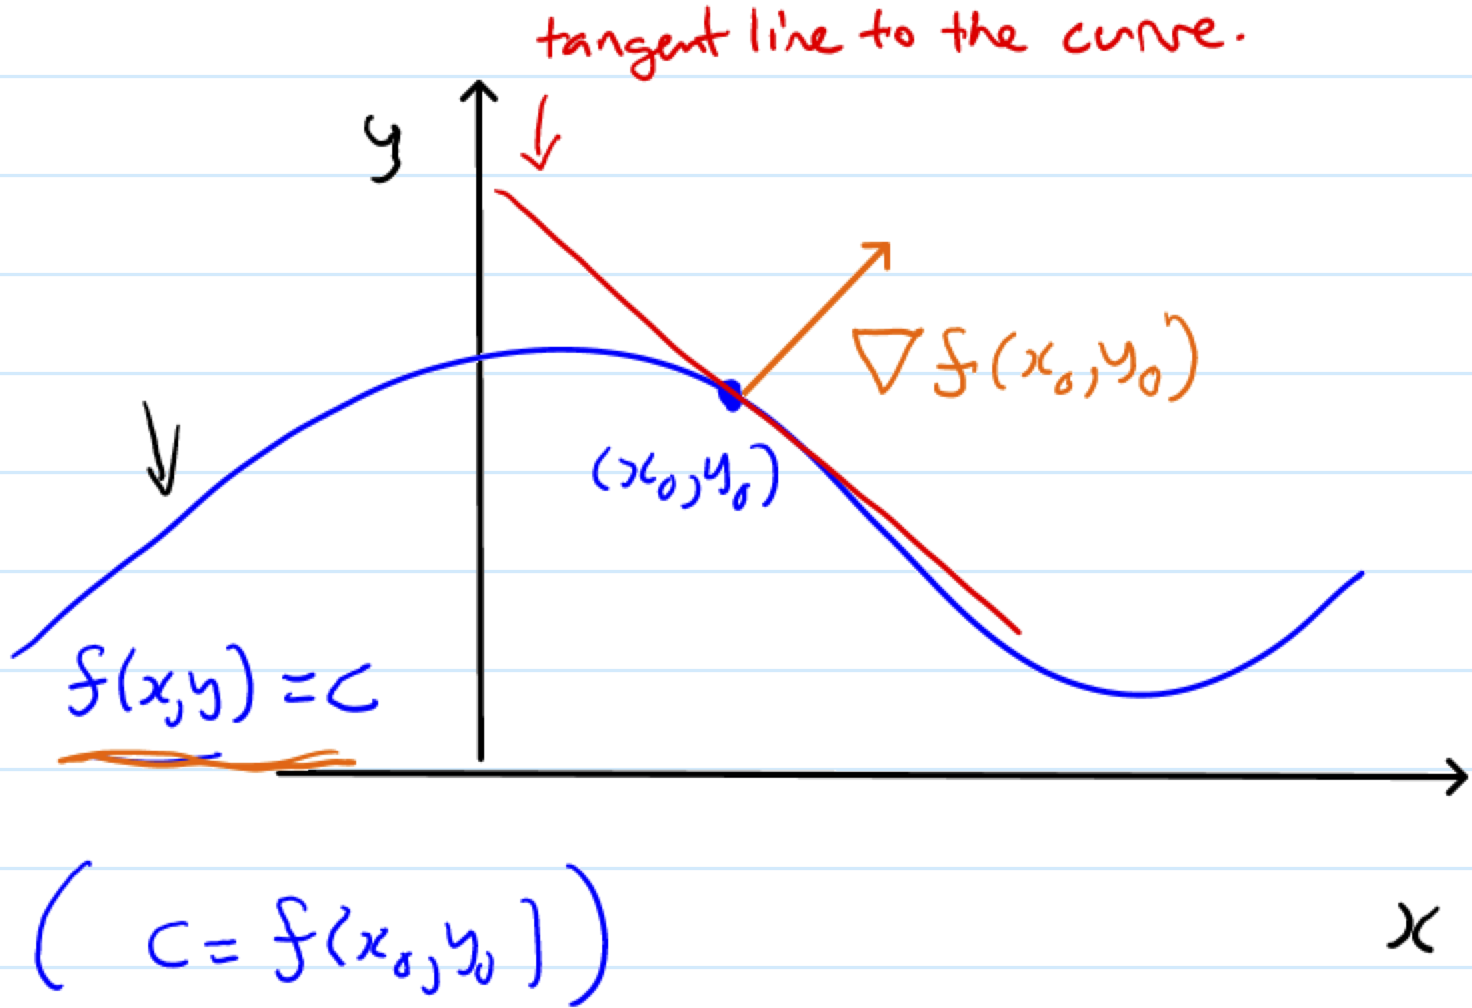
\includegraphics[scale=0.75]{derivative_level_curve} \end{center}

\subsubsection{Proof}
\[ \text{Let } \vec{r}(t) = (x(t), y(t)) \]
\[ \text{where } \vec{r}(0) = (x_0, y_0) \]
be a parametrisation of the level curve $f(x, y) = c = f(x_0, y_0)$.

Then
\[ f(\vec{r}(t)) = f(x(t), y(t)) = c \]
Differentiating with respect to $t$,
\begin{align*}
0 &= \left. \frac{d}{dt} \left( f(x(t), y(t)) \right) \right|_{t=0} \\
&= \left. \left( \frac{\partial f}{\partial x} (x(t), y(t)) \frac{\partial x}{\partial t}(t) + \frac{\partial f}{\partial y}(x(t), y(t)) \frac{\partial y}{\partial t}(t) \right) \right|_{t=0} \\
&= \frac{\partial f}{\partial x} (x_0, y_0) \frac{\partial x}{\partial t}(0) + \frac{\partial f}{\partial y}(x_0, y_0) \frac{\partial y}{\partial t}(0) \\
&= \nabla f(x_0, y_0) \cdot \frac{d\vec{r}}{dt}(0)
\end{align*}

Since $\dfrac{d\vec{r}}{dt}(0)$ is tangent to the level curve at the point $(x_0, y_0)$ and since its dot product with $\nabla f(x_0, y_0)$ is zero, we can conclude that the derivative of the function $f(x, y)$ at the point $(x_0, y_0)$ is orthogonal to the level curve passing through the point $(x_0, y_0)$

\end{document}